\documentclass[aspectratio=169,11pt]{beamer}

% --- Packages ---
\usepackage[utf8]{inputenc}
\usepackage[T1]{fontenc}
\usepackage{helvet}
\renewcommand{\familydefault}{\sfdefault}

\usepackage{graphicx}
\usepackage{booktabs}
\usepackage{array}
\usepackage{colortbl}
\usepackage{amsmath,amssymb}
\usepackage{tikz}
\usetikzlibrary{positioning,calc,shapes.geometric,decorations.pathmorphing,backgrounds,patterns}
\usepackage[many]{tcolorbox}
\usepackage{fontawesome5}
\usepackage{tabularx}
\usepackage{multicol}

% --- Beamer Settings ---
\usetheme{default}
\usecolortheme{default}
\setbeamertemplate{navigation symbols}{}
\setbeamertemplate{caption}{\insertcaption}

% --- Color Palette (Keynote Modern Dark & Light) ---
\definecolor{midnight}{HTML}{0F172A}      % Slate 900
\definecolor{navybg}{HTML}{1E293B}        % Slate 800
\definecolor{cardbg}{HTML}{F8FAFC}        % Slate 50
\definecolor{cardborder}{HTML}{E2E8F0}    % Slate 200
\definecolor{accentcyan}{HTML}{06B6D4}    % Cyan 500
\definecolor{accentblue}{HTML}{2563EB}    % Blue 600
\definecolor{accentpurple}{HTML}{7C3AED}  % Violet 600
\definecolor{textdark}{HTML}{0F172A}      % Slate 900
\definecolor{textmuted}{HTML}{64748B}     % Slate 500
\definecolor{textlight}{HTML}{94A3B8}     % Slate 400

% Apply default Beamer colors
\setbeamercolor{background canvas}{bg=white}
\setbeamercolor{normal text}{fg=textdark}
\setbeamercolor{framed}{fg=textdark}
\setbeamercolor{item}{fg=accentblue}

% --- Custom Keynote Card Style ---
\tcbset{
  keynotecard/.style={
    enhanced,
    colback=cardbg,
    colframe=cardborder,
    arc=4pt,
    boxrule=0.8pt,
    left=10pt,
    right=10pt,
    top=8pt,
    bottom=8pt,
    boxsep=0pt
  },
  darkcard/.style={
    enhanced,
    colback=navybg,
    colframe=accentcyan!40,
    arc=4pt,
    boxrule=0.8pt,
    left=10pt,
    right=10pt,
    top=8pt,
    bottom=8pt,
    boxsep=0pt
  },
  accentcard/.style={
    enhanced,
    colback=accentblue!8,
    colframe=accentblue!30,
    arc=4pt,
    boxrule=0.8pt,
    left=10pt,
    right=10pt,
    top=8pt,
    bottom=8pt,
    boxsep=0pt
  }
}

% --- Header and Footer Templates ---
\setbeamertemplate{frametitle}{
  \vspace*{8pt}
  \begin{minipage}{\textwidth}
    {\usebeamerfont{frametitle}\Large\bfseries\color{midnight}\insertframetitle}\par
    \ifx\insertframesubtitle\@empty\else
      \vspace*{2pt}
      {\usebeamerfont{framesubtitle}\tiny\color{textmuted}\insertframesubtitle}
    \fi
  \end{minipage}
  \vspace*{2pt}
}

\setbeamertemplate{footline}{
  \ifnum\insertpagenumber>1
    \vspace*{4pt}
    \begin{minipage}{\textwidth}
      \hspace*{20pt}%
      {\tiny\color{textlight}\bfseries MERIDIAN MEDIA LABS \hspace{6pt}\textperiodcentered\hspace{6pt} NEXT-GEN STREAMING STRATEGY}
      \hfill
      {\tiny\color{textlight}\insertframenumber\,/\,\inserttotalframenumber}
      \hspace*{20pt}%
    \end{minipage}
    \vspace*{8pt}
  \fi
}

% ==============================================================================
\begin{document}

% ------------------------------------------------------------------------------
% SLIDE 1: Title Slide (Full Bleed Dark Theme)
% ------------------------------------------------------------------------------
{
\setbeamercolor{background canvas}{bg=midnight}
\begin{frame}[plain]
  \vspace*{24pt}
  \begin{center}
    {\color{accentcyan}\large\bfseries\faTv\quad MERIDIAN MEDIA LABS} \par
    \vspace{14pt}
    {\fontsize{26pt}{32pt}\selectfont \color{white}\bfseries The Future of Digital Content} \par
    \vspace{8pt}
    {\fontsize{15pt}{20pt}\selectfont \color{accentcyan}\mdseries Scalable Ecosystems, AI Curation \& Next-Gen Distribution} \par
    \vspace{20pt}
    
\begin{tikzpicture}
      \draw[accentcyan, thick] (-2,0) -- (2,0);
    \end{tikzpicture}
    \vspace{20pt}
    
    {\small\color{textlight} Annual Media Technology Executive Briefing} \par
    \vspace{6pt}
    {\small\color{white}\bfseries Prepared by Elena Rostova \quad|\quad Head of Product Strategy} \par
    \vspace{4pt}
    {\tiny\color{textlight} Q3 Strategic Roadmap Presentation}
  \end{center}
\end{frame}
}

% ------------------------------------------------------------------------------
% SLIDE 2: Executive Summary
% ------------------------------------------------------------------------------
\begin{frame}{Executive Summary}{Transforming high-volume media delivery across global networks}
  \begin{center}
  \begin{minipage}{0.96\textwidth}
    \begin{tcolorbox}[keynotecard]
      {\mdseries\bfseries\color{accentblue}\faRocket\quad Key Strategic Objective} \par
      \vspace{2pt}
      \small\color{textdark} Meridian Media Labs is transitioning from legacy broadcast caching to a high-speed, personalized streaming infrastructure serving over \textbf{45 million daily active viewers}.
    \end{tcolorbox}
  \end{minipage}
  \end{center}
  
  \vspace{4pt}
  \begin{columns}[T]
    \begin{column}{0.31\textwidth}
      \begin{tcolorbox}[accentcard]
        \begin{center}
          {\huge\bfseries\color{accentblue} 3.8x} \par
          \vspace{2pt}
          {\small\bfseries Streaming Throughput} \par
          \vspace{2pt}
          {\tiny\color{textmuted} Year-over-year bandwidth optimization across 14 edge regions.}
        \end{center}
      \end{tcolorbox}
    \end{column}
    
    \begin{column}{0.31\textwidth}
      \begin{tcolorbox}[accentcard]
        \begin{center}
          {\huge\bfseries\color{accentpurple} 99.99\%} \par
          \vspace{2pt}
          {\small\bfseries Edge Reliability} \par
          \vspace{2pt}
          {\tiny\color{textmuted} Zero frame drops recorded during peak live sports broadcast.}
        \end{center}
      \end{tcolorbox}
    \end{column}
    
    \begin{column}{0.31\textwidth}
      \begin{tcolorbox}[accentcard]
        \begin{center}
          {\huge\bfseries\color{accentcyan} < 40ms} \par
          \vspace{2pt}
          {\small\bfseries Global Latency} \par
          \vspace{2pt}
          {\tiny\color{textmuted} Real-time content dynamic stitching at regional nodes.}
        \end{center}
      \end{tcolorbox}
    \end{column}
  \end{columns}
\end{frame}

% ------------------------------------------------------------------------------
% SLIDE 3: Table of Contents / Agenda
% ------------------------------------------------------------------------------
\begin{frame}{Agenda}{Key discussion areas for today's keynote}
  \vspace{2pt}
  \begin{columns}[T]
    \begin{column}{0.48\textwidth}
      \begin{tcolorbox}[keynotecard]
        \begin{minipage}{0.12\textwidth}
          {\Large\color{accentblue}\faGlobe}
        \end{minipage}%
        \begin{minipage}{0.85\textwidth}
          {\small\bfseries\color{textdark} 01. Global Market Context} \par
          {\tiny\color{textmuted} Shifting consumer habits \& high-bitrate demand}
        \end{minipage}
      \end{tcolorbox}
      \vspace{3pt}
      \begin{tcolorbox}[keynotecard]
        \begin{minipage}{0.12\textwidth}
          {\Large\color{accentblue}\faServer}
        \end{minipage}%
        \begin{minipage}{0.85\textwidth}
          {\small\bfseries\color{textdark} 02. Vertex Core Architecture} \par
          {\tiny\color{textmuted} Distributed CDN \& dynamic AI encoding pipeline}
        \end{minipage}
      \end{tcolorbox}
      \vspace{3pt}
      \begin{tcolorbox}[keynotecard]
        \begin{minipage}{0.12\textwidth}
          {\Large\color{accentblue}\faBrain}
        \end{minipage}%
        \begin{minipage}{0.85\textwidth}
          {\small\bfseries\color{textdark} 03. Synapse Curation Engine} \par
          {\tiny\color{textmuted} Context-aware recommendations \& real-time feeds}
        \end{minipage}
      \end{tcolorbox}
    \end{column}
    
    \begin{column}{0.48\textwidth}
      \begin{tcolorbox}[keynotecard]
        \begin{minipage}{0.12\textwidth}
          {\Large\color{accentpurple}\faChartLine}
        \end{minipage}%
        \begin{minipage}{0.85\textwidth}
          {\small\bfseries\color{textdark} 04. Engagement Metrics} \par
          {\tiny\color{textmuted} Audience retention metrics, AB test benchmarks}
        \end{minipage}
      \end{tcolorbox}
      \vspace{3pt}
      \begin{tcolorbox}[keynotecard]
        \begin{minipage}{0.12\textwidth}
          {\Large\color{accentpurple}\faCoins}
        \end{minipage}%
        \begin{minipage}{0.85\textwidth}
          {\small\bfseries\color{textdark} 05. Monetization \& AdTech} \par
          {\tiny\color{textmuted} Dynamic server-side ad insertion (SSAI)}
        \end{minipage}
      \end{tcolorbox}
      \vspace{3pt}
      \begin{tcolorbox}[keynotecard]
        \begin{minipage}{0.12\textwidth}
          {\Large\color{accentpurple}\faFlag}
        \end{minipage}%
        \begin{minipage}{0.85\textwidth}
          {\small\bfseries\color{textdark} 06. 2027 Strategic Roadmap} \par
          {\tiny\color{textmuted} Expansion phases, capital allocation, next steps}
        \end{minipage}
      \end{tcolorbox}
    \end{column}
  \end{columns}
\end{frame}

% ------------------------------------------------------------------------------
% SLIDE 4: Section Divider 1 (Full-Bleed Dark Accent)
% ------------------------------------------------------------------------------
{
\setbeamercolor{background canvas}{bg=midnight}
\begin{frame}[plain]
  \vspace*{36pt}
  \begin{minipage}{0.85\textwidth}
    {\color{accentcyan}\large\bfseries\faGlobe\quad SECTION 01} \par
    \vspace{12pt}
    {\fontsize{26pt}{32pt}\selectfont \color{white}\bfseries Shifting Media Paradigms} \par
    \vspace{8pt}
    {\fontsize{14pt}{18pt}\selectfont \color{textlight} Moving from static linear feeds to hyper-personalized, ultra-low latency streams.}
  \end{minipage}
  \vspace*{24pt}
  
\begin{tikzpicture}
    \fill[accentcyan] (0,0) rectangle (4,0.06);
  \end{tikzpicture}
\end{frame}
}

% ------------------------------------------------------------------------------
% SLIDE 5: Industry Trends & Market Challenge
% ------------------------------------------------------------------------------
\begin{frame}{Market Challenges}{3 critical pressures facing modern streaming platforms}
  \vspace{2pt}
  \begin{columns}[T]
    \begin{column}{0.31\textwidth}
      \begin{tcolorbox}[keynotecard]
        {\Large\color{accentblue}\faMobile} \par
        \vspace{4pt}
        {\bfseries\color{textdark} Multi-Device Support} \par
        \vspace{2pt}
        {\tiny\color{textmuted} Delivering consistent 4K 60fps HDR content seamlessly across TVs, mobile devices, and spatial displays.}
      \end{tcolorbox}
    \end{column}
    
    \begin{column}{0.31\textwidth}
      \begin{tcolorbox}[keynotecard]
        {\Large\color{accentblue}\faExclamationTriangle} \par
        \vspace{4pt}
        {\bfseries\color{textdark} Bandwidth Overhead} \par
        \vspace{2pt}
        {\tiny\color{textmuted} Peak global traffic demand spikes place severe load on regional origin servers during live broadcasts.}
      \end{tcolorbox}
    \end{column}
    
    \begin{column}{0.31\textwidth}
      \begin{tcolorbox}[keynotecard]
        {\Large\color{accentblue}\faUserClock} \par
        \vspace{4pt}
        {\bfseries\color{textdark} Retention \& Fatigue} \par
        \vspace{2pt}
        {\tiny\color{textmuted} Generic content feeds result in high churn rates. Viewers demand instantaneous discovery within 5 seconds.}
      \end{tcolorbox}
    \end{column}
  \end{columns}

  \vspace{6pt}
  \begin{tcolorbox}[accentcard]
    \small\color{textdark}\textbf{Industry Benchmark:} Platforms with latency exceeding 2.5 seconds experience an immediate \textbf{18\% drop} in session duration.
  \end{tcolorbox}
\end{frame}

% ------------------------------------------------------------------------------
% SLIDE 6: Section Divider 2 (Full-Bleed Dark Accent)
% ------------------------------------------------------------------------------
{
\setbeamercolor{background canvas}{bg=midnight}
\begin{frame}[plain]
  \vspace*{36pt}
  \begin{minipage}{0.85\textwidth}
    {\color{accentcyan}\large\bfseries\faServer\quad SECTION 02} \par
    \vspace{12pt}
    {\fontsize{26pt}{32pt}\selectfont \color{white}\bfseries Vertex Architecture} \par
    \vspace{8pt}
    {\fontsize{14pt}{18pt}\selectfont \color{textlight} End-to-end media pipeline engineered for high concurrency and resilience.}
  \end{minipage}
  \vspace*{24pt}
  
\begin{tikzpicture}
    \fill[accentcyan] (0,0) rectangle (4,0.06);
  \end{tikzpicture}
\end{frame}
}

% ------------------------------------------------------------------------------
% SLIDE 7: TikZ System Architecture Diagram
% ------------------------------------------------------------------------------
\begin{frame}{System Architecture}{End-to-end flow from ingest to edge playback}
  \begin{center}
  \begin{tikzpicture}[
    node distance=0.8cm and 0.8cm,
    block/.style={rectangle, draw=accentblue!80, fill=cardbg, thick, rounded corners=4pt, minimum height=1.0cm, minimum width=1.9cm, align=center, font=\tiny\bfseries},
    edgeblock/.style={rectangle, draw=accentcyan!80, fill=accentcyan!10, thick, rounded corners=4pt, minimum height=1.0cm, minimum width=1.9cm, align=center, font=\tiny\bfseries},
    line/.style={draw=accentblue, ->, >=stealth, thick}
  ]
    % Nodes
    \node (ingest) [block] {\faVideo\\[1pt] Ingest Gateway\\[1pt]\color{textmuted}RTMP / SRT};
    \node (encode) [block, right=of ingest] {\faCogs\\[1pt] Vertex Encoder\\[1pt]\color{textmuted}AV1 / HEVC};
    \node (synapse) [block, above=0.5cm of encode] {\faBrain\\[1pt] Synapse AI\\[1pt]\color{textmuted}Metadata \& Tags};
    \node (origin) [block, right=of encode] {\faDatabase\\[1pt] Origin Shield\\[1pt]\color{textmuted}Object Storage};
    \node (edge) [edgeblock, right=of origin] {\faBroadcastTower\\[1pt] Edge CDN\\[1pt]\color{textmuted}240+ Locations};
    \node (client) [block, right=of edge] {\faDesktop\\[1pt] Client Devices\\[1pt]\color{textmuted}Smart TV / Mobile};

    % Connections
    \draw[line] (ingest) -- (encode);
    \draw[line] (encode) -- (origin);
    \draw[line] (origin) -- (edge);
    \draw[line] (edge) -- (client);
    \draw[line, dashed, color=accentpurple] (synapse) -- (encode);
    \draw[line, dashed, color=accentpurple] (synapse) -| (edge);
  \end{tikzpicture}
  \end{center}
  
  \vspace{4pt}
  \begin{columns}[T]
    \begin{column}{0.48\textwidth}
      \begin{tcolorbox}[keynotecard]
        {\small\bfseries\color{accentblue}\faCheckCircle\quad Dynamic Transcoding} \par
        {\tiny\color{textmuted} Adapts bitrates in real-time based on network telemetry and client hardware capabilities.}
      \end{tcolorbox}
    \end{column}
    \begin{column}{0.48\textwidth}
      \begin{tcolorbox}[keynotecard]
        {\small\bfseries\color{accentblue}\faCheckCircle\quad Edge Intelligence} \par
        {\tiny\color{textmuted} Synapse AI manifests personalized ad breaks and thumbnail previews directly at the edge POP.}
      \end{tcolorbox}
    \end{column}
  \end{columns}
\end{frame}

% ------------------------------------------------------------------------------
% SLIDE 8: Performance Metrics (Table)
% ------------------------------------------------------------------------------
\begin{frame}{Performance Benchmark}{Comparative trial results across key deployment regions}
  \vspace{2pt}
  \centering
  \resizebox{0.92\textwidth}{!}{%
  \begin{tabular}{l c c c c}
    \toprule
    \textbf{Deployment Region} & \textbf{Peak Traffic} & \textbf{Legacy Latency} & \textbf{Vertex Latency} & \textbf{Bandwidth Savings} \\
    \midrule
    North America (US-East) & 14.2 Tbps & 180 ms & \textbf{32 ms} & 34.2\% \\
    Europe (EU-Central) & 11.8 Tbps & 210 ms & \textbf{38 ms} & 31.8\% \\
    Asia Pacific (AP-Tokyo) & 9.4 Tbps & 240 ms & \textbf{41 ms} & 29.5\% \\
    Latin America (SA-East) & 4.1 Tbps & 320 ms & \textbf{54 ms} & 38.0\% \\
    \bottomrule
  \end{tabular}%
  }

  \vspace{8pt}
  \begin{columns}[T]
    \begin{column}{0.48\textwidth}
      \begin{tcolorbox}[accentcard]
        {\bfseries\color{accentblue}\faChartBar\quad Global Latency Drop} \par
        \vspace{2pt}
        {\tiny\color{textmuted} Average latency decreased by \textbf{81\%} following the deployment of Vertex Origin Shield.}
      \end{tcolorbox}
    \end{column}
    
    \begin{column}{0.48\textwidth}
      \begin{tcolorbox}[accentcard]
        {\bfseries\color{accentpurple}\faDollarSign\quad Infrastructure Efficiency} \par
        \vspace{2pt}
        {\tiny\color{textmuted} AV1 neural encoding generated \textbf{\$4.2M} in annual cloud bandwidth cost reductions.}
      \end{tcolorbox}
    \end{column}
  \end{columns}
\end{frame}

% ------------------------------------------------------------------------------
% SLIDE 9: Section Divider 3 (Full-Bleed Dark Accent)
% ------------------------------------------------------------------------------
{
\setbeamercolor{background canvas}{bg=midnight}
\begin{frame}[plain]
  \vspace*{36pt}
  \begin{minipage}{0.85\textwidth}
    {\color{accentcyan}\large\bfseries\faBrain\quad SECTION 03} \par
    \vspace{12pt}
    {\fontsize{26pt}{32pt}\selectfont \color{white}\bfseries Synapse Curation Engine} \par
    \vspace{8pt}
    {\fontsize{14pt}{18pt}\selectfont \color{textlight} Deep neural recommendations driving viewer engagement and session length.}
  \end{minipage}
  \vspace*{24pt}
  
\begin{tikzpicture}
    \fill[accentcyan] (0,0) rectangle (4,0.06);
  \end{tikzpicture}
\end{frame}
}

% ------------------------------------------------------------------------------
% SLIDE 10: Deep Feature Spotlight (Synapse AI)
% ------------------------------------------------------------------------------
\begin{frame}{Synapse AI Engine}{Personalized media recommendations at sub-second speeds}
  \begin{columns}[T]
    \begin{column}{0.48\textwidth}
      \begin{tcolorbox}[keynotecard]
        {\bfseries\color{accentblue}\faDraftingCompass\quad Contextual Vectors} \par
        \vspace{4pt}
        {\tiny\color{textmuted} Evaluates user viewing patterns, time of day, device category, and historical velocity to build dynamic recommendation lists.}
      \end{tcolorbox}
      \vspace{4pt}
      \begin{tcolorbox}[keynotecard]
        {\bfseries\color{accentblue}\faLayerGroup\quad Real-Time Tagging} \par
        \vspace{4pt}
        {\tiny\color{textmuted} Computer vision algorithms scan incoming broadcast frames to index scenes, actors, and brand appearances automatically.}
      \end{tcolorbox}
    \end{column}
    
    \begin{column}{0.48\textwidth}
      \begin{tcolorbox}[darkcard]
        {\bfseries\color{accentcyan}\faTerminal\quad Synapse Core Metrics} \par
        \vspace{6pt}
        \begin{itemize}
          \setlength{\itemsep}{4pt}
          \item[{\color{accentcyan}\faAngleRight}] {\small\color{white}\textbf{Recommendation Latency:} < 12ms}
          \item[{\color{accentcyan}\faAngleRight}] {\small\color{white}\textbf{CTR Increase:} +42.4\% vs. baseline}
          \item[{\color{accentcyan}\faAngleRight}] {\small\color{white}\textbf{Daily Model Updates:} Every 6 hours}
          \item[{\color{accentcyan}\faAngleRight}] {\small\color{white}\textbf{Active Features:} 1,200+ signals}
        \end{itemize}
      \end{tcolorbox}
    \end{column}
  \end{columns}
\end{frame}

% ------------------------------------------------------------------------------
% SLIDE 11: Keynote Quote / Callout (Full Bleed Accent)
% ------------------------------------------------------------------------------
{
\setbeamercolor{background canvas}{bg=navybg}
\begin{frame}[plain]
  \vspace*{28pt}
  \begin{center}
    {\fontsize{48pt}{48pt}\selectfont \color{accentcyan}“} \par
    \vspace{-16pt}
    \begin{minipage}{0.85\textwidth}
      \centering
      {\fontsize{18pt}{24pt}\selectfont \color{white}\itshape The future of media belongs to platforms that eliminate the friction between discovery and instantaneous playback.}
    \end{minipage} \par
    \vspace{18pt}
    
\begin{tikzpicture}
      \draw[accentcyan, thick] (-1.5,0) -- (1.5,0);
    \end{tikzpicture}
    \vspace{12pt}
    
    {\bfseries\color{white} Marcus Vance} \par
    {\small\color{textlight} Chief Technology Officer, Meridian Media Group}
  \end{center}
\end{frame}
}

% ------------------------------------------------------------------------------
% SLIDE 12: Monetization & AdTech Platform
% ------------------------------------------------------------------------------
\begin{frame}{Monetization \& AdTech}{Seamless server-side ad insertion (SSAI) with zero latency impact}
  \begin{columns}[T]
    \begin{column}{0.48\textwidth}
      \begin{tcolorbox}[keynotecard]
        {\bfseries\color{accentpurple}\faBullhorn\quad Dynamic SSAI Integration} \par
        \vspace{4pt}
        {\tiny\color{textmuted} Ad markers are stitched directly into the HLS/DASH manifest at edge nodes. Eliminates client-side ad blocker interruptions.}
        \vspace{6pt}
        \begin{itemize}
          \setlength{\itemsep}{2pt}
          \item[{\small\color{accentpurple}\faCheck}] {\tiny Frame-accurate ad insertion}
          \item[{\small\color{accentpurple}\faCheck}] {\tiny Zero buffering between ad \& content}
          \item[{\small\color{accentpurple}\faCheck}] {\tiny Real-time impression auditing}
        \end{itemize}
      \end{tcolorbox}
    \end{column}
    
    \begin{column}{0.48\textwidth}
      \begin{tcolorbox}[accentcard]
        \begin{center}
          {\huge\bfseries\color{accentpurple} \$18.50} \par
          \vspace{2pt}
          {\small\bfseries Average eCPM Rate} \par
          \vspace{2pt}
          {\tiny\color{textmuted} +34\% lift compared to client-side ad calls}
        \end{center}
      \end{tcolorbox}
      \vspace{2pt}
      \begin{tcolorbox}[accentcard]
        \begin{center}
          {\huge\bfseries\color{accentblue} 98.6\%} \par
          \vspace{2pt}
          {\small\bfseries Ad Completion Rate} \par
          \vspace{2pt}
          {\tiny\color{textmuted} High viewer retention during broadcast breaks}
        \end{center}
      \end{tcolorbox}
    \end{column}
  \end{columns}
\end{frame}

% ------------------------------------------------------------------------------
% SLIDE 13: Strategic Roadmap (TikZ Timeline)
% ------------------------------------------------------------------------------
\begin{frame}{2026 -- 2027 Strategic Roadmap}{Phase-by-phase rollout plan for next-gen deployment}
  \vspace{6pt}
  \begin{center}
  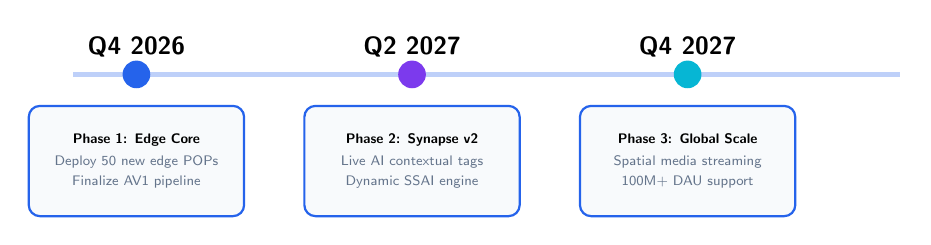
\begin{tikzpicture}[
    stage/.style={rectangle, draw=accentblue, fill=cardbg, thick, rounded corners=4pt, text width=2.5cm, minimum height=1.4cm, align=center, font=\tiny},
    arrowline/.style={->, >=stealth, ultra thick, accentblue}
  ]
    % Timeline line
    \draw[line width=2pt, accentblue!30] (0,0) -- (10.5,0);
    
    % Milestone 1
    \fill[accentblue] (0.8,0) circle (5pt);
    \node at (0.8, 0.35) {\small\bfseries Q4 2026};
    \node at (0.8,-1.1) [stage] {\textbf{Phase 1: Edge Core}\\[2pt]\color{textmuted} Deploy 50 new edge POPs\\[1pt] Finalize AV1 pipeline};
    
    % Milestone 2
    \fill[accentpurple] (4.3,0) circle (5pt);
    \node at (4.3, 0.35) {\small\bfseries Q2 2027};
    \node at (4.3,-1.1) [stage] {\textbf{Phase 2: Synapse v2}\\[2pt]\color{textmuted} Live AI contextual tags\\[1pt] Dynamic SSAI engine};
    
    % Milestone 3
    \fill[accentcyan] (7.8,0) circle (5pt);
    \node at (7.8, 0.35) {\small\bfseries Q4 2027};
    \node at (7.8,-1.1) [stage] {\textbf{Phase 3: Global Scale}\\[2pt]\color{textmuted} Spatial media streaming\\[1pt] 100M+ DAU support};
  \end{tikzpicture}
  \end{center}
  
  \vspace{10pt}
  \begin{tcolorbox}[keynotecard]
    \small\color{textdark}\textbf{Key Milestone Target:} Complete migration of all North American and European tier-1 traffic to Vertex Origin Shield by \textbf{June 2027}.
  \end{tcolorbox}
\end{frame}

% ------------------------------------------------------------------------------
% SLIDE 14: Action Items & Strategic Next Steps
% ------------------------------------------------------------------------------
\begin{frame}{Strategic Next Steps}{Key focus areas for executive leadership}
  \vspace{2pt}
  \begin{columns}[T]
    \begin{column}{0.48\textwidth}
      \begin{tcolorbox}[keynotecard]
        {\small\bfseries\color{accentblue}\faHdd\quad Capital Investment} \par
        \vspace{2pt}
        {\tiny\color{textmuted} Allocate \$12.5M for edge infrastructure expansion across Latin America and APAC growth hubs.}
      \end{tcolorbox}
      \vspace{3pt}
      \begin{tcolorbox}[keynotecard]
        {\small\bfseries\color{accentblue}\faHandshake\quad Content Partner Integration} \par
        \vspace{2pt}
        {\tiny\color{textmuted} Onboard Nexa Media \& Apex Studios onto the Synapse SDK platform by Q1 2027.}
      \end{tcolorbox}
    \end{column}
    
    \begin{column}{0.48\textwidth}
      \begin{tcolorbox}[keynotecard]
        {\small\bfseries\color{accentpurple}\faLock\quad Security \& DRM Enhancement} \par
        \vspace{2pt}
        {\tiny\color{textmuted} Implement dynamic forensic watermarking to prevent unauthorized redistribution of live events.}
      \end{tcolorbox}
      \vspace{3pt}
      \begin{tcolorbox}[keynotecard]
        {\small\bfseries\color{accentpurple}\faUsers\quad Talent Acquisition} \par
        \vspace{2pt}
        {\tiny\color{textmuted} Expand the distributed engineering team by hiring 15 specialized video system architects.}
      \end{tcolorbox}
    \end{column}
  \end{columns}
\end{frame}

% ------------------------------------------------------------------------------
% SLIDE 15: Closing Slide (Full Bleed Dark Theme)
% ------------------------------------------------------------------------------
{
\setbeamercolor{background canvas}{bg=midnight}
\begin{frame}[plain]
  \vspace*{36pt}
  \begin{center}
    {\fontsize{32pt}{38pt}\selectfont \color{white}\bfseries Thank You} \par
    \vspace{10pt}
    {\fontsize{15pt}{20pt}\selectfont \color{accentcyan} Building the Next Generation of Media Technology} \par
    \vspace{24pt}
    
\begin{tikzpicture}
      \draw[accentcyan, thick] (-2,0) -- (2,0);
    \end{tikzpicture}
    \vspace{24pt}
    
    {\small\color{white}\bfseries Meridian Media Labs} \par
    \vspace{4pt}
    {\small\color{textlight}\faEnvelope\quad strategy@meridianmedialabs.com \quad|\quad \faGlobe\quad www.meridianmedialabs.com}
  \end{center}
\end{frame}
}

\end{document}
